\title{IIT Bhubaneswar BTP Template}
\author{Srikanta}
\date{December 2020}

\documentclass[12pt]{report}
\usepackage[utf8]{inputenc}
\usepackage{listings}
\usepackage{xcolor}
% styling separately code
\documentclass{article}
\usepackage{listings}

\usepackage{xcolor}

%New colors defined below
\definecolor{codegreen}{rgb}{0,0.6,0}
\definecolor{codegray}{rgb}{0.5,0.5,0.5}
\definecolor{codepurple}{rgb}{0.58,0,0.82}
\definecolor{backcolour}{rgb}{0.95,0.95,0.92}

%Code listing style named "mystyle"
\lstdefinestyle{mystyle}{
  backgroundcolor=\color{backcolour}, commentstyle=\color{codegreen},
  keywordstyle=\color{magenta},
  numberstyle=\tiny\color{codegray},
  stringstyle=\color{codepurple},
  basicstyle=\ttfamily\footnotesize,
  breakatwhitespace=false,         
  breaklines=true,                 
  captionpos=b,                    
  keepspaces=true,                 
  numbers=left,                    
  numbersep=5pt,                  
  showspaces=false,                
  showstringspaces=false,
  showtabs=false,                  
  tabsize=2
}


%additional packages
\usepackage{amsmath}
\usepackage{lipsum}
\usepackage{graphicx}
\usepackage{caption}
\usepackage{subcaption}
\usepackage{longtable}
\graphicspath{{figures/}}
\usepackage[a4paper,width=160mm,top=25mm,bottom=25mm]{geometry}
\usepackage{titlesec}
\linespread{1.2}
\usepackage{subcaption}
\usepackage{schemabloc,tikz}
\usepackage{amsfonts,epsfig,cite,array,multirow,graphicx,amsmath,amsthm,ltablex,tabularx,setspace,arydshln,amssymb,multirow}
\usetikzlibrary{circuits, arrows}
\newtheorem{theorem}{Theorem}
\newtheorem{lemma}{Lemma}
\usepackage[utf8]{inputenc}
\usepackage{amsmath}
\usepackage{amsfonts}
\usepackage{amssymb}
\usepackage{bbm}
\usepackage{mathtools}
\usepackage{textcomp}
\usepackage{stackengine}
\usepackage{booktabs}
\usepackage{longtable}
\usepackage{multirow}
\usepackage{graphicx}
\usepackage{subcaption}

\def\mytitle{Comparable Attribute-Based
Encryption Construction with 0-Encoding
and 1-Encoding}
\def\myname{Ankit Patel}
\def\degree{Bachelor of Technology}
\def\mydegree{Computer Science and Engineering}
\def\mysupervisor{Dr. Padmalochan Bera}
\def\myrollno{20CS01009}
\def\mydep{School of Electrical Sciences}

\begin{document}

%Front Matter
\thispagestyle{empty}
\begin{center}
\vspace*{0.5cm}
    { \Large {\bfseries {\mytitle}} \par}
\vspace{2\baselineskip}
    {\textit{Project-I (CS4D001) Report submitted in partial fulfillment for}\\
    \textit{the award of degree of}}\par
\vspace{0.2\baselineskip}
    {\bf \degree \par}
\vspace{0.2\baselineskip}
    {\textit{in} \par}
\vspace{0.2\baselineskip}
    {\Large \bf \mydegree \par} 
\vspace{\baselineskip}
    {\textit{by} \par}
\vspace{\baselineskip}
    {{\Large {\bf \myname \\ \myrollno}} \par}
\vspace{1.5\baselineskip}
    {\large Under the supervision of \par}
\vspace{0.3\baselineskip}
    {{\Large \bf \mysupervisor} \par}
\vspace{\baselineskip}
    {\begin{figure}[!h] 
	\centering
	
\includegraphics[width=60mm]{./Images/Logo.png} 
     \end{figure}
    }
    \vspace{1.5\baselineskip}
    {\large \MakeUppercase{\mydep} \par}
\vspace*{2ex}
    {\large \uppercase{Indian Institute of Technology Bhubaneswar} \par}
\end{center}
 \pagenumbering{roman}
\chapter*{Declaration}

I affirm that the project titled \textbf{“Comparable Attribute-Based
Encryption Construction with 0-Encoding
and 1-Encoding”}, submitted for the partial fulfillment of the requirements for the Degree of Bachelor of Technology in Computer Science Engineering at the Indian Institute of Technology Bhubaneswar, within the School of Electrical Sciences, is a genuine representation of my independent work conducted between July 2023 and November 2023 under the supervision of \textbf{Dr. Padmalochan Bera}, IIT Bhubaneswar.
\\
\\
I declare that the content presented in this project has not been previously submitted for the attainment of any degree at this or any other Institute/University.
\\
\\
\\
\begin{flushright}
    \textbf{Ankit Patel (20CS01009)}
\end{flushright}
This certification attests that the aforementioned statement by the candidate is accurate to the best of our knowledge.
\\
\\
\\
\begin{flushright}
    \textbf{Signature of Supervisor}
\end{flushright}

\addcontentsline{toc}{chapter}{Declaration}
\chapter*{Abstract}
\hspace{10mm}Attribute-based encryption (ABE) has opened up a popular research topic in cryptography over the past few years. It can be
used in various circumstances, as it provides a flexible way to conduct fine-grained data access control. Despite its great advantages in
data access control, current ABE based access control system cannot satisfy the requirement well when the system judges the access
behavior according to attribute comparison, such as “greater than x” or “less than x”, which are called comparable attributes in this
paper. In this paper, based on a set of well-designed sub-attributes representing each comparable attribute, we construct a comparable
attribute-based encryption scheme (CABE for short) to address the aforementioned problem. The novelty lies in that we provide a more
efficient construction based on the generation and management of the sub-attributes with the notion of 0-encoding and 1-encoding.
Extensive analysis shows that: Compared with the existing schemes, our scheme drastically decreases the storage, communication
and computation overheads, and thus is more efficient in dealing with the applications with comparable attributes. Related implementation and theory have been mentioned further in the report as well.

\addcontentsline{toc}{chapter}{Abstract}
\tableofcontents
% \listoffigures
% \listoftables

%Chapters
\clearpage
 \pagenumbering{arabic}
\chapter{Introduction}

\section{Background}

\hspace{10mm}
In an era dominated by unprecedented volumes of digital data and an ever-expanding threat landscape, the imperative to secure sensitive information has never been more critical. Traditional encryption methods, while effective in many scenarios, often fall short when it comes to managing access to data in complex, dynamic environments. In response to these challenges, Attribute-Based Encryption (ABE) emerges as a revolutionary paradigm, offering a nuanced and flexible approach to data protection.

ABE represents a departure from conventional encryption models by enabling access control based on attributes rather than traditional cryptographic keys or passwords. This innovative cryptographic technique provides a granular and adaptive means of securing information, aligning more closely with the intricacies of modern data-sharing scenarios. There are several algorithms for ABE like KP-ABE and CP-ABE.

In several distributed systems a user should only be able to access data if a user possesses a certain set of credentials or attributes. Currently, the only method for enforcing such policies is to employ a trusted server to store the data and mediate access control. However, if any server storing the data is compromised, then the confidentiality of the data will be compromised. Ciphertext-policy attribute-based encryption presents a system for realizing complex access control on encrypted data that we call. By using these techniques encrypted data can be kept confidential even if the storage server is untrusted; moreover, these methods are secure against collusion attacks. Previous attribute-based encryption systems used attributes to describe the encrypted data and built policies into user's keys; while in the system attributes are used to describe a user's credentials, and a party encrypting data determines a policy for who can decrypt. Thus, these methods are conceptually closer to traditional access control methods such as role-based access control .
Ciphertext-policy attribute-based encryption (CP-ABE) to address this problem, and give the first construction of such a scheme. In the system,a user’s private key will be associated with an arbitrary number of attributes expressed as strings. On the other hand, when a party encrypts a message in our system, they specify an associated access structure over attributes. A user will only be able to decrypt a ciphertext if that user’s attributes pass through the ciphetext’s access structure. At a mathematical level, access structures in our system are described by a monotonic “access tree”, where nodes of the access structure are composed of threshold gates and the leave describe attributes. We note that AND gates can be constructed as n-of-n threshold gates and OR gates as 1-of-n threshold gates. Furthermore, we can handle more complex access controls such as numeric ranges by converting them to small access trees 
\section{Encryption}
The process of converting the original representation of the information, known as plaintext into an alternative form known as cipher-text. Modern encryption schemes use the concepts of public-key and symmetric-key. 
In symmetric-key schemes, the encryption and decryption keys are the same. Communicating parties must have the same key in order to achieve secure communication. In public-key encryption schemes, the encryption key is published for anyone to use and encrypt messages. However, only the receiving party has access to the decryption key that enables messages to be read. 
           
\section{Fine-grained Access Control}
Fine-grained access control systems facilitate granting differential access rights to a set of users and allow flexibility in specifying the access rights of individual users. Identity-Based Encryption (IBE) is a cryptographic scheme that is related to the concepts of fine-grained access control.

\section{Identity Based Encryption}
Identity based encryption is a type of public-key encryption in which the public key of a user is some unique information about the identity of the user (e.g. a user's email address). This means that a sender who has access to the public parameters of the system can encrypt a message. The receiver obtains its decryption key from a central authority, which needs to be trusted as it generates secret keys for every user. 

\begin{figure}[h]
    \centering
   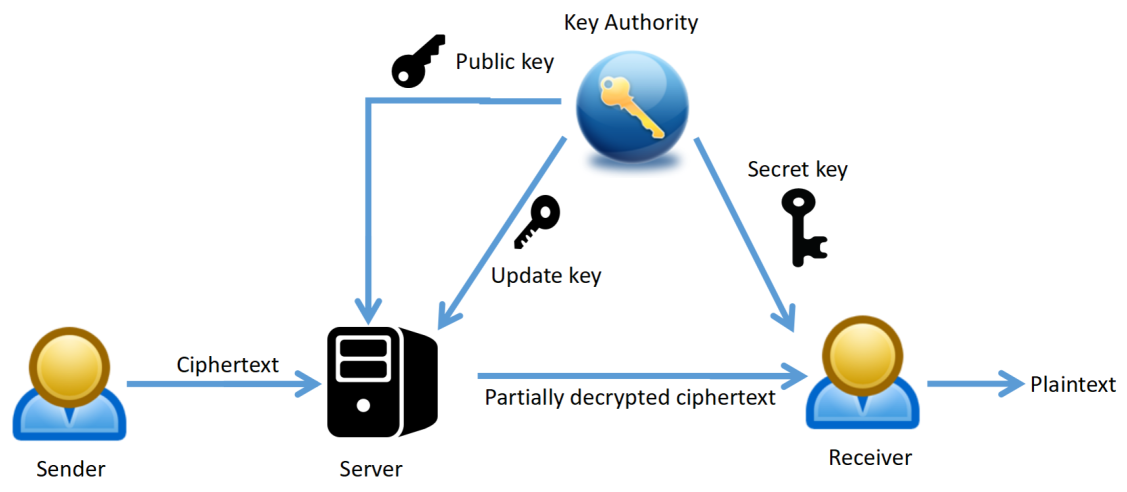
\includegraphics[width=\linewidth]{Images/IBEV2.png}
    \caption{Example of Identity Based Encryption}
    \label{fig:enter-label}
\end{figure}

\section{Attribute Based Encryption}
Attribute-based encryption is probably a generalization of identity-based encryption which enables fine grained access control of encrypted data using authorisation policies. The secret key of a user and the ciphertext are dependent upon attributes (e.g. their email address, the country in which they live, or the kind of subscription they have). In such a system, the decryption of a ciphertext is possible only if the set of attributes of the user key matches the attributes of the ciphertext.Researchers have further proposed attribute-based encryption with multiple authorities who jointly generate users' private keys. There are mainly two types of attribute-based encryption schemes: Key-policy attribute-based encryption (KP-ABE) and ciphertext-policy attribute-based encryption (CP-ABE).
An important property which has to be achieved by both, CP-ABE and KP-ABE is called collusion resistance. If multiple users try to access the encrypted data, they should only be able to decrypt a ciphertext if at least one of the users could decrypt it on their own. Both CP-ABE and KP-ABE provide Collusion Resistance.
\section{Access Policies}
Access policies refer to rules that govern the permissions and restrictions placed on entities attempting to access cryptographic resources. Here are some types of access policies commonly used:
\begin{itemize}

    \item\bm AND-Gate Policy: This policy requires that a user possesses all specified attributes for access.

    \item\bm OR-Gate Policy: An OR-Gate policy allows access if a user possesses at least one of the specified attributes.

\end{itemize}
\begin{figure}
    \centering
   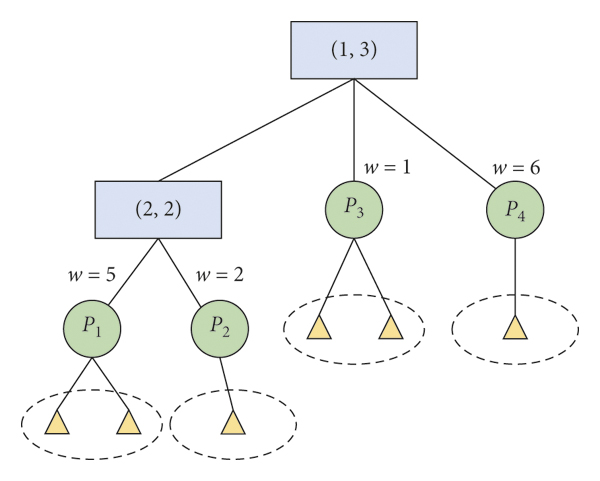
\includegraphics[width=\linewidth]{Images/ABE.png}
    \caption{Example of Attribute Based Encryption}
    \label{fig:enter-label}
\end{figure}
\begin{figure}
    \centering
   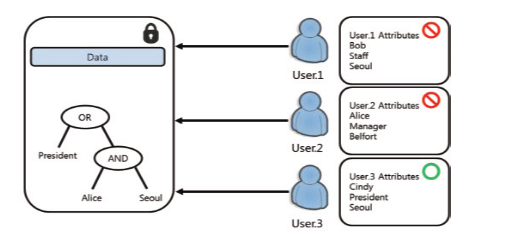
\includegraphics[width=\linewidth]{Images/ANDOR.png}
    \caption{Example of Attribute Based Encryption}
    \label{fig:enter-label}
\end{figure}
\chapter{CipherText Policy Attribute Based Encryption}

% \section{Literature Review}


In ciphertext-policy attribute-based encryption (CP-ABE) ,a user's private key will be associated with an arbitrary number of attributes expressed as strings,from the universe of attributes available. 
On the other hand, when a party encrypts a message in our system, they specify an associated access structure over attributes. A user will only be able to decrypt a ciphertext if that user’s attributes pass through the ciphertext’s access structure. 


   At a mathematical level, access structures in our system are described by a monotonic “access tree”, where nodes of the access structure are composed of threshold gates and the leaves describe attributes. We note that AND gates can be constructed as n-of-n threshold gates and OR gates as 1-of-n threshold gates. Furthermore, we have implemented more complex access controls such as numeric ranges by converting them to smaller access trees using 0-1 Encoding for comparison.
\begin{figure}
    \centering
    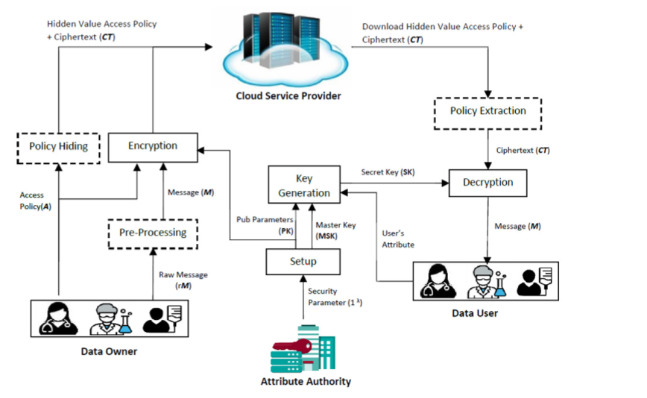
\includegraphics[width=0.8\linewidth]{Images/CBCArchitecture.jpeg}
    \caption{Standard Archicture of CP-ABE}
    \label{fig:enter-label}
\end{figure}
    A ciphertext-policy attribute based encryption scheme consists of four fundamental algorithms: Setup, Encrypt, KeyGen, and Decrypt. In addition, we allow for the option of a fifth algorithm Delegate.

    \begin{enumerate}
    \item Setup\par
 The setup algorithm takes no input other than the implicit security parameter. It outputs the public parameters PK and a master key MK.
    \item Encrypt(PK,M, A)\par
   The encryption algorithm takes as input the public parameters PK, a message M, and an access structure A over the universe of attributes. The algorithm will encrypt M and produce a ciphertext CT such that only a user that possesses a set of attributes that satisfies the access structure will be able to decrypt the message. We will assume that the ciphertext implicitly contains A.
    \item Key Generation(MK,S)\par
   The key generation algorithm takes as input the master key MK and a set of attributes S that describe the key. It outputs a private key SK.
    \item Encrypt(PK,M, A) \par
   The encryption algorithm takes as input the public parameters PK, a message M, and an access structure A over the universe of attributes. The algorithm will encrypt M and produce a ciphertext CT such that only a user that possesses a set of attributes that satisfies the access structure will be able to decrypt the message. We will assume that the ciphertext implicitly contains A.
    \item Decrypt(PK, CT, SK) \par
  The decryption algorithm takes as input the public parameters PK, a ciphertext CT, which contains an access policy A, and a private key SK, which is a private key for a set S of attributes. If the set S of attributes satisfies the access structure A then the algorithm will decrypt the ciphertext and return a message M.
  \item Delegate(SK, S ̃) \par
 The delegate algorithm takes as input a secret key SK for some set of attributes S and a set S ̃⊆ S. It output a secret key SK for the set of  ̃ attributes S ̃.
\end{enumerate}






\chapter{ The Problem}


In the current implementation for the CP-ABE include only AND and OR gates which allows us to define the access policy based on them for example : ((“Public Corruption Office” AND (“Knoxville” OR “San Francisco”)) OR(management-level > 5) OR “Name: CharlieEppes”).
However, AND gate alone cannot designate intended users well in many cases. Thus the schemes supporting threshold gates have been attracting much more attention. An encryption and decryption algorithm with fewer participating attributes and less complex policies is preferred. The cost increases linearly with the attribute number. However, the value comparison in access policy should expand the attribute number of the structure. Thus, an inefficient mechanism may affect the feasibility of the scheme. 
\\

\noindent \textbf{Objective:}\par
The comparison operation between a user’s and a file’s attributes only includes “=”.These attributes are numerical information,and will probably be used in comparison. For instance, a user may be assigned a key embedded with access policy as: “(Distance \(<\) 1000 miles) AND (Date \(>\)  May 1st)” For example, “Distance \(<\) 1000 miles” can be represented as a formula like (“Distance = 999 miles” or “Distance = 998 miles”  or  ... “Distance = 0 miles”), but the overhead increases linearly with the growth of attribute’s value space, which will become a performance bottleneck of the system. This scheme divided such numerical attribute into pieces in units of bits as several sub-attributes to solve this problem. However, the mechanism to design a numeric-comparison policy is too complex, and the most essential problem is that the additional overhead is still relatively high in both Space and Time.




\chapter{ Proposed Solution}


In there paper by (Kaiping Xue, Senior Member, IEEE,), they proposed a new scheme to enable ABE to implement comparable attributes, called Comparable Attribute-based Encryption (CABE). In CABE, we  use a unique way to generate and manage sub-attributes for comparable attributes, so as to make a solution for addressing the above issue in an efficient way, in terms of both storage overhead and computation overhead. Our solution in dealing with sub-attributes are based on a special notion called 0-encoding and 1-encoding. The main contributions of this paper can be summarized as follows:
\begin{enumerate}
    \item We propose an efficient method based on a special concept 0-encoding and 1-encoding, so that the attributes can be used in arbitrary comparison, which is suitable for ABE system;
     \item A lightweight and efficient CABE construction is proposed. This construction halves the expanded storage overhead in average compared with related schemes, and significantly decreases the computation overhead in encryption and decryption from O(log n) to O(1) (N denotes the value space of the attribute dimension).
\end{enumerate}
\textbf{
\section{Definition of 0-Encoding and 1-Encoding}
}
Our system uses the concept of two special encodings, 0-encoding and 1-encoding.
Let 
\[{s = s_ns_{n-1} \ldots s_1 \in \{0,1\}^n}\]

 be an n-length binary string of a value for a certain attribute dimension. 

\begin{itemize}
    \item The 0-encoding of s is defined as a set such that \[{ S^0_s\ = \{ {s}_ns_{n-1} \ldots s_{i+1}1|s_i = 0,1<=i<=n \} } \]
     \item The 1-encoding of s is defined as a set such that \[{ S^0_s\ = \{ {s}_ns_{n-1} \ldots s_{i}|s_i = 1,1<=i<=n \} } \]
\end{itemize}
Intuitively, 1-encoding of s is the set of all its odd prefix substrings, and the 0-encoding is the set of all of its modified even prefix substrings, where the least significant bit is flipped from “0” to “1”. The size of set S0s equals to the number of characters “0” in string s, and meanwhile the size of S1s equals to the number of “1”. 
Compared with the value space of n-length binary string: N=2n, both S1s and S0s have at most log N elements. To compare two integers x and y in the form of n-length binary string, we encode x into 1-encoding  and into 0-encoding \(S_0^y\)  . We make the judgment that \[ x > y \] if and only if there’s an element in both \(S_1^x\) and \(S_0^y\)  . A formula to express this theorem is as

\begin{figure}[h]
    \centering
    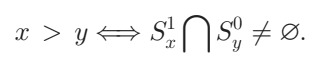
\includegraphics[width=0.3\linewidth]{Images/IntersectionOfSets.jpeg}
   
\end{figure}

\begin{figure}[h]
    \centering
    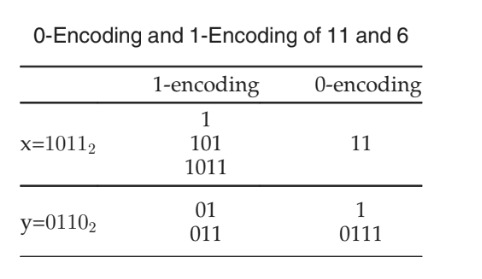
\includegraphics[width=0.7\linewidth]{Images/01EncodingTable.jpeg}
   
\end{figure}

\textbf{
\section{Storing of 0-Encoding and 1-Encoding}
}
The object we deal with is such an attribute that is not an exact value, but stands as a range of continuous values, and may be matched in comparison in the ABE system, such as “\(Score > 75\)”, “\(Age < 25\)”. For one attribute field F, whose value space is N and minimum value is \(val_{min}\), we can reduce the storage overhead to ½(\(log_2N)\) on average to make this kind of attribute suit  CP-ABE construction with utilization of 0-encoding and 1-encoding. Our procedure is implemented as follows  For a value x  F, if its minimum value is not zero, compute 
\(x_m\)=x - \(val_{min}\);
otherwise, such operations can be skipped. For clarity of description, let \(x_m\)=x; in this case. If the length of the binary string \(x_m\) is less than \(log_2N\), use 0 to fill at high bits. Then what the program deals with is a new \(log_2N\)-long binary string \(x_m\). We encode \(x_m\) into 0-encoding \(S_0\)
\(x_m\) and 1-encoding S1 \(x_m\) with the rule described in Section 3.1. For a certain access structure, if the access policy needs the corresponding attribute F to satisfy that \(F > x\), an attribute set \(Set_{c0}\)(F,x) can be designed as . A formula to express this theorem is as

\begin{figure}[h]
    \centering
    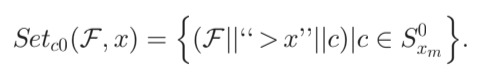
\includegraphics[width=0.6\linewidth]{Images/ConcatenationOfConditions.jpeg}
   
\end{figure}

\begin{figure}[h]
    \centering
    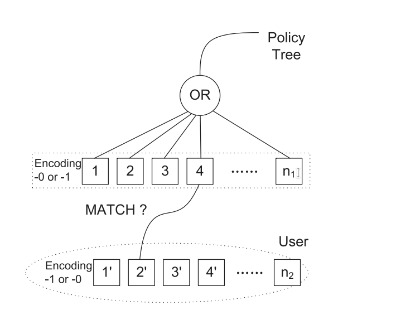
\includegraphics[width=0.7\linewidth]{Images/TreeOrMatching.jpeg}
   
\end{figure}



\textbf{
\section{Proposed Range Query Solution}
}
Since we already exposed the mathematical construct on how to reduce the numerical comparison to simple binary AND and OR operations we will now propose our solution for efficient range query. Some lemmas must be mentioned before proposing our solution : 
\begin{itemize}
    \item \textbf{
    Lemma 1 : Encode a into its 0-Encoding set  \(E_0\) and b into its 1-encoding set \(E_1\) , we have \(b > a\) if and only if \(E_1\) and \(E_0\) have some elements in common.
    }
    \item From this lemma we can derive the theorem that the common element will be a single element.
    A further observation that can be made from this is that if there is no common element between the 2 sets then \(b<=a\). 

\end{itemize}
Now in our solution we decided to perform some operations on the access policy with the range comparisons such that the intersection of the 2 0-Encoding and 1-Encoding set can be left up to the access policy tree itself and it will perform the intersection on the elements in 2 sets using the binary operations. This is done using the logic that say we want to find the intersection between 2 sets say set A and set B then if say we have 1 encoding of set A , the individual elements of 1 - encoding of the set can be taken in the form A1 OR A2 OR A3 OR A4 which are nothing but the individual elements of the 1-encoding. 

Now say we get an actual value to compare then we can calculate it’s 0-encoding and push that itself in the access tree and tell our access tree to perform the intersection function by doing comparison of individual elements thus resulting in intersection of the 2 sets of 1- Encoding of A and 0-Encoding of B and if access tree returns 1 that is true then it has found an element in intersection and thus we have successfully calculated that \(b < a\).

Similarly we can swap the encoding schemes for integers and get the result 
 “ \(x > value\) “ 
Now to implement the negation comparison for an attribute like “ \(x!= value\)  ” we decided to do a deep dive in boolean logic along with set theory and for the given conditions we came up with the solution that if “ \(x < value or x > value \) ” returns a 0 value that means \(x != value\) . Proof for this lies in the fact that if \(x == value \)then \(x < value\) returns None and \(x > value\) returns None and if we take \(None OR None\) we get\(None\)  aka \(0 aka False\). Now any number except value can be \(either >\) value or \(< value\) where the condition “ \( x < value or x > value \) ” will return true hence the negation condition can be implemented successfully. So we were able to implement range based comparison by combining the 2 conditions like “\(x < a and x > b \)“ such that “\(x belongs to ( b,a )\)”  and “ \(x<a or x >a \)” implying “ \(x!=a\) ”.

Hence we were able to efficiently implement range based comparison in the access tree compared to previously known inefficient method which basically involved iterating through all the numbers in a given range \(( 1,n )\) such that it performed equality check on all individual numbers in the given range thus becoming increasingly inefficient when the range of numbers became very big as inherent complexity of that is \(O(n)\) in both time as well as more complexity in space due to overhead of maintaining the access structure as well.


In our proposed solution and implementation we have cut down the time complexity from \(O (N)\) to \(O (log N)\)  and space complexity to \(O (log N)\) as well, which we will demonstrate via some benchmarking graphs that we calculated on our code.









\lstdefinestyle{mystyle}{
    language=Python,
    basicstyle=\ttfamily\small,
    commentstyle=\color{green!40!black},
    keywordstyle=\color{blue},
    numberstyle=\tiny\color{gray},
    numbers=left,
    frame=single,
    breaklines=true,
    showstringspaces=false,
    captionpos=b,
    tabsize=4
}

\chapter{Charm Crypto Library And My Contribution}
\section{Required Auxillary Functions}

To do this we have defined some auxiliary functions over existing charm crypto library whose screen shots have been attached below :
\begin{itemize}
    \item \textbf{def encode\_number} : is a function that returns the 0-Encoding and 1-Encoding of a number which is used further to perform the binary comparison for 2 numbers.
    \item \textbf{def modify\_access\_policy} : is a function that takes input the access policy with comparable range comparisons and performs the required replacements with the given 0 and 1 attribute sets such that the binary comparison can be performed by the access structure in our tree.
    \item \textbf{def modify\_not\_equal\_condition} : is a function that is responsible for implementing the \(a !=b \) operation using the preexisting range comparison operators whose maths has been previously explained.
\end{itemize}



\begin{lstlisting}[style=mystyle, caption={Encode Number Function}, label=yourlabel]

# In each of the 0-encoding and 1-encoding sets, E0
# a and E1
# b , the binary strings are arranged in the
# decreasing order of string length (i.e., the number of digits of a binary sequence)


def encode_number(x):
    # Convert the integer to a binary string
    binary_string = bin(x)[2:]

    # Pad the binary string with leading zeros if needed
    # standardize all binary strings to be of length 32
    binary_string = binary_string.zfill(32)
    # Initialize 0-encoding and 1-encoding sets
    S0_x = set()
    S1_x = set()

    # Iterate over the binary string and populate the sets
    for i in range(len(binary_string)):
        prefix = binary_string[:i+1]
        if prefix[-1] == '0':
            # Flip the least significant bit when adding to S0_x
            S0_x.add(prefix[:-1] + '1')
        else:
            S1_x.add(prefix)
    # convert the binary to decimal
    # sort S0_x and S1_x by length of the binary string
    S0_x = sorted(S0_x, key=lambda x: len(x), reverse=True)
    S1_x = sorted(S1_x, key=lambda x: len(x), reverse=True)
    return S0_x, S1_x

\end{lstlisting}



\begin{lstlisting}[style=mystyle, caption={Function for implementing a!=b operator}, label=yourlabel]

def modify_not_equal_conditions(access_policy):
    pattern = re.compile(r'(\w+)\s*(!=)\s*(\d+)')
    matches = pattern.findall(access_policy)
    for match in matches:
        identifier, operator, number = match
        S0_x, S1_x = encode_number(int(number))
        new_condition = f'({identifier} < {number} OR {identifier} > {number})'
        access_policy = access_policy.replace(
            f'{identifier} {operator} {number}', new_condition)
    return access_policy
\end{lstlisting}
\begin{lstlisting}[style=mystyle, caption={Function for modifying access policy for Range comparison}, label=yourlabel]
def modify_access_policy(access_policy):
    access_policy = modify_not_equal_conditions(access_policy)
    pattern = re.compile(r'(\w+)\s*([<>])\s*(\d+)')
    matches = pattern.findall(access_policy)
    for match in matches:
        identifier, operator, number = match
        access_policy = access_policy.replace(
            f'{identifier} {operator} {number}', f'({identifier} {operator} {number})')
    matches = pattern.findall(access_policy)
    for match in matches:
        identifier, operator, number = match
        S0_x, S1_x = encode_number(int(number))
        if operator == '<':
            new_condition = ' OR '.join(f'{identifier}{"!!"}{x}' for x in S1_x)
        elif operator == '>':  # operator == '>'
            new_condition = ' OR '.join(f'{identifier}{"@@"}{x}' for x in S0_x)
        access_policy = access_policy.replace(
            f'({identifier} {operator} {number})', f'({new_condition})')
    pattern = re.compile(r'(\w+) = (\w+)')
    modified_policy = access_policy
    for match in pattern.findall(access_policy):
        old_expression = f'{match[0]} = {match[1]}'
        new_expression = f'({match[0]}$${match[1]})'
        new_expressionx = new_expression.upper()
        modified_policy = modified_policy.replace(
            old_expression, new_expressionx)
    return modified_policy
\end{lstlisting}
\begin{lstlisting}[style=mystyle, caption={Function for modifying attributes for range comparison}, label=yourlabel]
def process_attributes(attributes):
    pattern = re.compile(r'(\w+) = (\d+)')
    for i, attribute in enumerate(attributes):
        match = pattern.match(attribute)
        if match:
            attr_name = match.group(1).upper()
            attr_value = int(match.group(2))
            S0_attr, S1_attr = encode_number(attr_value)
            attr_encodings = [f'{attr_name}!!{x}' for x in S0_attr] + \
                [f'{attr_name}@@{x}' for x in S1_attr]
            attributes[i:i+1] = attr_encodings
    pattern = re.compile(r'(\w+) = (\w+)')
    for i, attribute in enumerate(attributes):
        match = pattern.match(attribute)
        if match:
            old_expression = attribute
            # capitalize the new_expression
            new_expression = f'{match[1]}$${match[2]}'
            new_expressionx = new_expression.upper()
            attributes[i] = new_expressionx
    return attributes


\end{lstlisting}

\chapter{Result and Analysis}

\section{Parameters for comparison}
3 kinds of graphs have been primarily used to evaluate the performance of our proposed  algorithm which are 

\begin{itemize}
    \item \textbf{Key Generation Time} : This represents the amount of time the algorithm takes to generate the public key and the secret key based on the access policy size .
 \item \textbf{Encryption Time} : This represents the amount of time it takes to encrypt a given generic text file which can be examined while looking at our code .
  \item \textbf{Decryption Time} : This represents the amount of time it takes to decrypt a given encrypted document so as to get the original information.
\end{itemize}

\subsection{Range Value Comparison}
Theoretical calculations and graphs also have been provided along with our own benchmarks so as to show case the efficiencies of our algorithm. The most important graph can be the key generation symmetric and decryption time vs the actual range because our whole solution is about optimizing the extremely big numerical ranges compared to the generic implementation of CP-ABE which are extremely slow and memory hogging for moderately big values of numbers. Now lets’ observe the graphs obtained for extremely large value of ranges which were implemented in the access policy of the form  \(x < range1 \)  and   \(x > range2\) .

\begin{figure}[h]
    \centering
    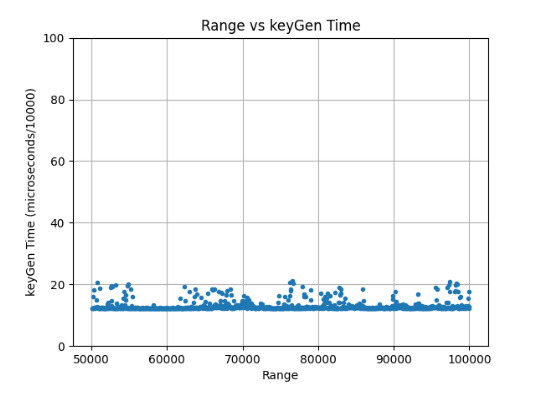
\includegraphics[width=0.75\linewidth]{Images/RangeVsKeyGen.jpeg}
    \caption{Range vs Time Taken For key generation}
    \label{fig:enter-label}
\end{figure}


\begin{figure}[h]
    \centering
    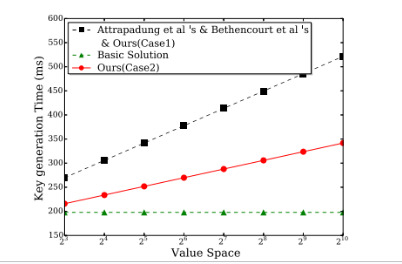
\includegraphics[width=0.75\linewidth]{Images/RangeVsKeyGenTheoritical.jpeg}
    \caption{Range vs Time Taken For key generation Theoritical}
    \label{fig:enter-label}
\end{figure}

An extremely slow growing almost constant \(O(1)\) complexity is observed in the time consumption for the keyGen algorithm which proves that our algorithm is way faster than the generic implementation of range queries for CP-ABE which is \(O(N)\) in nature which blows up very quickly in terms of memory as well as time required for calculations.
This almost constant time complexity is in line with the theoretical calculations that were proved in the paper that was used for reference.


\subsection{Access Length Comparison}
We observe that the time taken for Key Generation remains pretty much constant irrespective of the access policy length which is in line with our assumption that irrespective of the fact that how big the number of attributes get the growth is extremely slow approximately log (n) or barely constant. 
Similar graphs can be drawn for encryption and decryption time which can be used to draw some conclusions about the various optimisation techniques that can be used in the decrypting process which can be observed in the next page.
In case of attribute length as  a parameter which represents the number of parameters present in the user who is trying to decrypt the encrypted file and linearly increasing but stable relationship is observed between the key generation time and number of parameters in Attribute for a given user.

\begin{figure}[h]
    \centering
    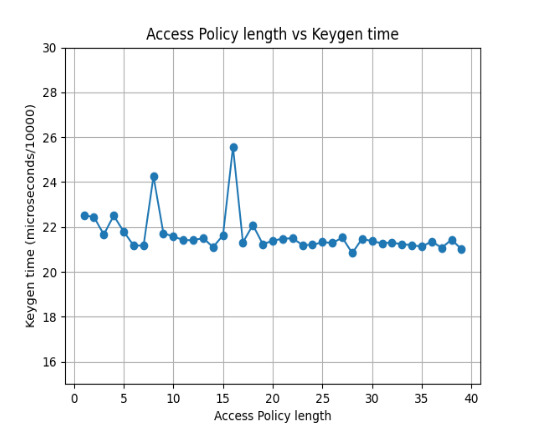
\includegraphics[width=0.75\linewidth]{Images/AccessPolicyLengthVsKeyGenTime.jpeg}
 
    \caption{Access Policy Length vs Time Taken For key generation }
    \label{fig:enter-label}
\end{figure}


\begin{figure}
    \centering
    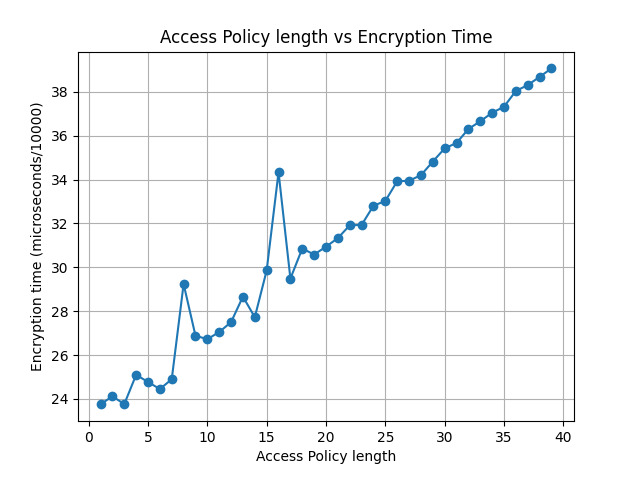
\includegraphics[width=0.75\linewidth]{Images/AccessPolicyLengthVsEncryptionTime.jpeg}
    \caption{Access Policy Length vs Encryption Time }
    \label{fig:enter-label}
\end{figure}


\begin{figure}
    \centering
    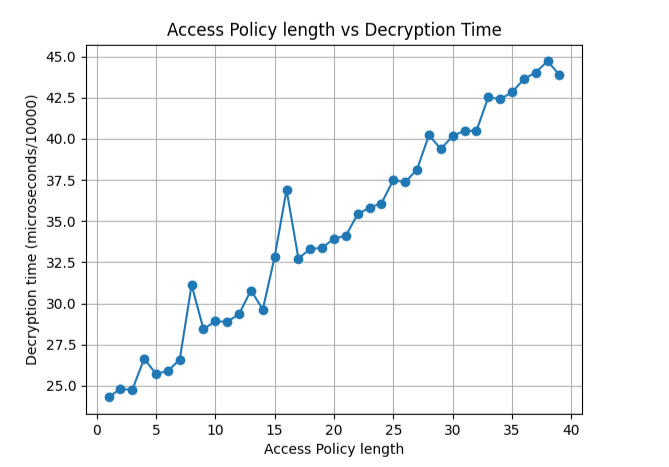
\includegraphics[width=0.75\linewidth]{Images/AccessPolicyVsDecryptionTime.jpeg}
    \caption{Access Policy Length vs Encryption Time }
    \label{fig:enter-label}
\end{figure}


\subsection{Attribute Length Comparison}
In case of attribute length as  a parameter which represents the number of parameters present in the user who is trying to decrypt the encrypted file and linearly increasing but stable relationship is observed between the key generation time and number of parameters in Attribute for a given user.
Some uniformity is observed in the encryption algorithm where as some non linearity can be observed in the decryption algorithm which is due to varying level of optimisations being performed with the given access structure and given attribute properties array for the user attempting to decrypt the file.
Some uniformity is observed in the encryption algorithm where as some non linearity can be observed in the decryption algorithm which is due to varying level of optimisations being performed with the given access structure and given attribute properties array for the user attempting to decrypt the file.

\begin{figure}[h]
    \centering
    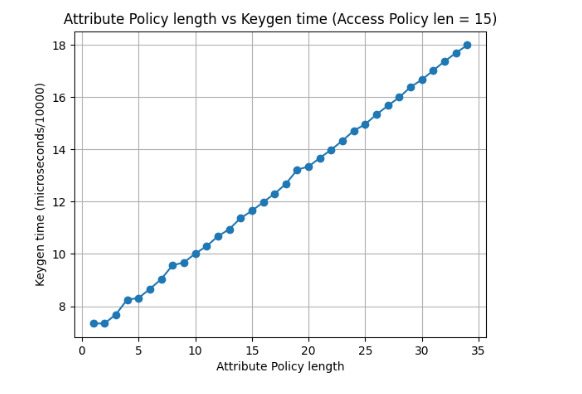
\includegraphics[width=0.75\linewidth]{Images/AttributeLenghtVsKeyGen.jpeg}
 
    \caption{Attribute Policy Length vs Time Taken For key generation }
    \label{fig:enter-label}
\end{figure}


\begin{figure}
    \centering
    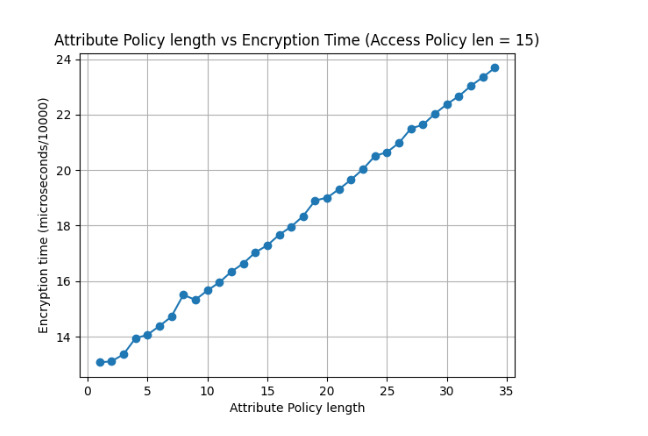
\includegraphics[width=0.75\linewidth]{Images/AttributeLenghtVsEncryptionTime.jpeg}
    \caption{Attribute Policy Length vs Encryption Time }
    \label{fig:enter-label}
\end{figure}


\begin{figure}
    \centering
    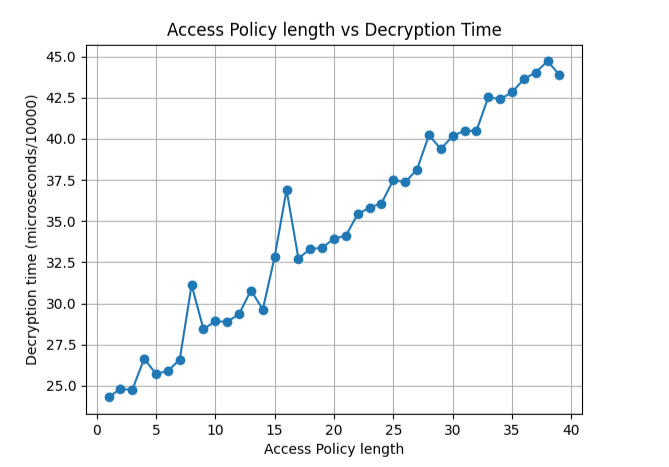
\includegraphics[width=0.75\linewidth]{Images/AccessPolicyVsDecryptionTime.jpeg}
    \caption{Attribute Policy Length vs Encryption Time }
    \label{fig:enter-label}
\end{figure}

\lstdefinestyle{mystyle}{
    language=Python,
    basicstyle=\ttfamily\small,
    commentstyle=\color{green!40!black},
    keywordstyle=\color{blue},
    numberstyle=\tiny\color{gray},
    numbers=left,
    frame=single,
    breaklines=true,
    showstringspaces=false,
    captionpos=b,
    tabsize=4
}

\chapter{Sample Code For Encrypting a text file}

\begin{lstlisting}[style=mystyle, caption={Sample Code For Ecrypting a File}, label=yourlabel]
import random
from charm.toolbox.pairinggroup import PairingGroup
from charm.schemes.abenc.abenc_bsw07 import CPabe_BSW07
from charm.adapters.abenc_adapt_hybrid import HybridABEnc
import pickle
import time
import re
#assumed function definitions given previously
def test(access_policy_len, extra_attribute_lenght, rangeNum1, rangeNum2):
    start_time = time.time()
    groupObj = PairingGroup('SS512')
    cpabe = CPabe_BSW07(groupObj)
    hyb_abe = HybridABEnc(cpabe, groupObj)
    (pk, mk) = hyb_abe.setup()
    access_policy = '((four and three) and (two or one) and (ran != 120) and (age < 25 and age > 10))'
    # access_policy = f'(age < {rangeNum2}  and age > {rangeNum1})'
    # print("RANGE BEING USED IN ACCESS_POLICY", rangeNum1, rangeNum2)
    # print("ACCESS POLICY LENGTH : ", access_policy_len,
        #   " ATTRIBUTE POLICY LENGHT : ", extra_attribute_lenght)
    new_access_policy = modify_access_policy(access_policy)
    # benchmark_access_policy = modify_access_policyx(
        # new_access_policy, access_policy_len)
    # print(benchmark_access_policy)
    # print(modify_access_policyx(access_policy), "ok")
    attributes = ['ONE', 'TWO', 'THREE','Prof',
                  'FOUR', 'ran = 121', 'age = 24', 'collegeTeacher = XYZ']
    # attributes = [f'age = {(rangeNum1+rangeNum2)//2}']
    # print(attributes,access_policy)
    # attributes = generate_attributes(
        # benchmark_access_policy, extra_attribute_lenght)
    processed_attributes = process_attributes(attributes)
    # print(len(processed_attributes),len(benchmark_access_policy),benchmark_access_policy)
    print(processed_attributes, "X")
    print(new_access_policy,'new Access policy')
    # print(processed_attributes,'new processedd attributes')
    sk = hyb_abe.keygen(pk, mk, processed_attributes)
    # print(len(attributes), "len")
    keygen_time = time.time() - start_time
    print("Keygen time: ", keygen_time*1e6, " microseconds")
    sourcefile = open("source.txt", 'rb')
    plaintext = sourcefile.read()
    sourcefile.close()

    encryptedfile = open("encrypted.txt", 'wb')
    ciphertext = hyb_abe.encrypt(pk, plaintext, new_access_policy)
    # ciphertext = hyb_abe.encrypt(pk, plaintext, benchmark_access_policy)
    encryption_time = time.time() - start_time
    print("Encryption time: ", encryption_time*1e6, " microseconds")
    ciphertext["c1"]["C"] = groupObj.serialize(ciphertext["c1"]["C"])
    for key in ciphertext["c1"]["Cy"]:
        ciphertext["c1"]["Cy"][key] = groupObj.serialize(
            ciphertext["c1"]["Cy"][key])
    ciphertext["c1"]["C_tilde"] = groupObj.serialize(
        ciphertext["c1"]["C_tilde"])
    for key in ciphertext["c1"]["Cyp"]:
        ciphertext["c1"]["Cyp"][key] = groupObj.serialize(
            ciphertext["c1"]["Cyp"][key])
    pickle.dump(ciphertext, encryptedfile)
    encryptedfile.close()

    encryptedfile = open("encrypted.txt", 'rb')
    ciphertext2 = pickle.load(encryptedfile)
    ciphertext2["c1"]["C"] = groupObj.deserialize(ciphertext2["c1"]["C"])
    for key in ciphertext2["c1"]["Cy"]:
        ciphertext2["c1"]["Cy"][key] = groupObj.deserialize(
            ciphertext2["c1"]["Cy"][key])
    ciphertext2["c1"]["C_tilde"] = groupObj.deserialize(
        ciphertext2["c1"]["C_tilde"])
    for key in ciphertext2["c1"]["Cyp"]:
        ciphertext2["c1"]["Cyp"][key] = groupObj.deserialize(
            ciphertext2["c1"]["Cyp"][key])
    try :
        print(hyb_abe.decrypt(pk, sk, ciphertext2), plaintext)
        ans = hyb_abe.decrypt(pk, sk, ciphertext2)
    except :    
        return
    decryption_time = time.time() - start_time
    print("Decryption time: ", decryption_time*1e6, " microseconds")
    encryptedfile.close()


if __name__ == "__main__":
    debug = True
    # for i in range(1,42):
        # test(i,0,0,0)
        # print('*'*30)
    # for i in range(1, 100000,50):
        # if 1e5-i > i:
            # test(1, i, i, 100000-i)
            # print('*'*30)
    # for i in range(1, 35):
        # test(15, i, 23, 23)
        # print('*'*30)
    test(0,0,0,0)
\end{lstlisting}

\chapter*{Conclusion}


The presented work addresses the limitations of traditional Cipher Policy Attribute-Based Encryption (CP-ABE) systems by introducing a novel scheme known as Comparable Attribute-Based Encryption (CABE). This scheme efficiently handles comparable attributes in access policies, offering improvements in both storage and computation overhead. The key contributions of this work include the introduction of 0-encoding and 1-encoding concepts, a lightweight CABE construction, and an efficient method for managing sub-attributes.

The utilization of 0-encoding and 1-encoding provides an innovative approach to handle arbitrary comparisons in ABE systems.
The 0-encoding and 1-encoding sets are defined based on the binary representation of values, enabling efficient comparison operations.
Lightweight CABE Construction:

The proposed CABE construction demonstrates a significant reduction in storage overhead compared to related schemes.
\begin{itemize}
    \item Average storage overhead is reduced by half, and encryption/decryption computation overhead is reduced from O(log n) to O(1).
    \item \textbf{ Definition of 0-Encoding and 1-Encoding } : The definitions of 0-encoding and 1-encoding are clearly articulated, providing a foundation for the efficient management of comparable attributes.
    \item \textbf{ Efficient Range Query Solution: } : TThe proposed solution for efficient range queries leverages the mathematical constructs of 0-encoding and 1-encoding. Through the use of access policy trees and binary operations, the system efficiently performs range-based attribute comparisons.
      \item \textbf{ Negation Comparison Implementation } : The implementation effectively handles negation comparisons by combining conditions and exploiting boolean logic.
       \item \textbf{ Range-based Comparison } : Range-based comparisons, such as  \( x<a\) and  \(x>b\), are efficiently integrated into the access tree.
         \item \textbf{ Benchmarking Results: } : Through benchmarking, the proposed solution demonstrated a substantial reduction in time and space complexity compared to traditional methods. The time complexity was reduced from O(N) to O(log N), and the space complexity was similarly reduced to O(log N)

\end{itemize}











\addcontentsline{toc}{chapter}{Conclusion}
\chapter*{Future Work}

In the forthcoming stages of project, we plan to:
\begin{itemize}
  \item Make it an independent self deployable service by any person or organisation:
  \begin{itemize}
      \item The project aims to improve upon the existing code base and the pre existing solutions.
      \item Using containerizing technologies like docker and making it an independent web server we plan on make it a self hostable encrypted FTP server on which user can upload a file and can specify the access policy and then people with required credentials can access the FTP server and decrypt the data if their attributes satify the access policy.
  \end{itemize}
  \item Implement another efficient comparison algorithm and make it deployable on IoT devices:
  \begin{itemize}
      \item In the research papers that we came across while pursuing this project we came across some new algorithms which are even more efficient time and space wise compared to our solution which can be implemented and make the whole encryption process even more efficient and thus make it deployable on plethora of IoT devices..
  \end{itemize}
\end{itemize}


\addcontentsline{toc}{chapter}{Future Work}
\bibliographystyle{IEEEtran}
\begin{thebibliography}{99}
\bibitem{Qx1}John Bethencourt Amit Sahai  Brent Waters. \textit{Ciphertext-Policy Attribute-Based Encryption} Carnegie Mellon University , UCLA , SRI International.
\bibitem{Qx2}Kaiping Xue ,Jianan Hong, Yingjie Xue,David S. L. Wei,Nenghai Yu, and Peilin Hong. \textit{CABE: A New Comparable Attribute-Based
Encryption Construction with 0-Encoding
and 1-Encoding } 
\bibitem{Qx3}PING YU, WEI NI,
REN PING LIU, 
ZHAOXIN ZHANG,
HUA ZHANG and QIAOYAN WEN,
\textit{Efficient Encrypted Range Query on Cloud Platforms} Faculty of Computing, Harbin Institute of Technology
, Commonwealth Scientific and Industrial Research Organization (CSIRO) Sydney
, University of Technology Sydney
, Faculty of Computing, Harbin Institute of Technology
, State Key Laboratory of Networking and Switching Technology,
Beijing University of Posts and Telecommunications.

\end{thebibliography}
\addcontentsline{toc}{chapter}{References}
\end{document}

% \input{Chapters/Literature}
% \addcontentsline{toc}{chapter}{Literature Study}
% \include{./Chapters/Applications}
\chapter{ The Problem}


In the current implementation for the CP-ABE include only AND and OR gates which allows us to define the access policy based on them for example : ((“Public Corruption Office” AND (“Knoxville” OR “San Francisco”)) OR(management-level > 5) OR “Name: CharlieEppes”).
However, AND gate alone cannot designate intended users well in many cases. Thus the schemes supporting threshold gates have been attracting much more attention. An encryption and decryption algorithm with fewer participating attributes and less complex policies is preferred. The cost increases linearly with the attribute number. However, the value comparison in access policy should expand the attribute number of the structure. Thus, an inefficient mechanism may affect the feasibility of the scheme. 
\\

\noindent \textbf{Objective:}\par
The comparison operation between a user’s and a file’s attributes only includes “=”.These attributes are numerical information,and will probably be used in comparison. For instance, a user may be assigned a key embedded with access policy as: “(Distance \(<\) 1000 miles) AND (Date \(>\)  May 1st)” For example, “Distance \(<\) 1000 miles” can be represented as a formula like (“Distance = 999 miles” or “Distance = 998 miles”  or  ... “Distance = 0 miles”), but the overhead increases linearly with the growth of attribute’s value space, which will become a performance bottleneck of the system. This scheme divided such numerical attribute into pieces in units of bits as several sub-attributes to solve this problem. However, the mechanism to design a numeric-comparison policy is too complex, and the most essential problem is that the additional overhead is still relatively high in both Space and Time.




\addcontentsline{toc}{chapter}{Problem Statement}